\label{sec:empirical}
% Empirical	Approach
% Description of the empirical model: specification and variables involved
% Strategy for the estimation of the parameters of interest and test of the hypothesis
\subsection{Network Characteristics}
When analyzing the network we utilize the \texttt{NetworkX} package in Python. We start by characterizing the network. Recall, that we view airports as nodes, and flights between airports as edges. Considering the dataset of flights in 2018 from the Bureau of Transportation Statistics, we produce a network of US airports and the flights connecting them. We will refer to this network as the US Network. This network has 358 nodes and 3220 edges. With 310 nodes, the maximum possible number of edges would be (\cite{Barabasi Networks}): 
\begin{align}
    L_{max}  = \frac{N\cdot(N-1)}{2}=\frac{358\cdot(358-1)}{2} = 63.903
\end{align}
This implies, that only approximately 5 pct. of possible edges are actually found in the network. 
% Tjek nedenstående når vi ved mere
This sparseness of the network supports the hub-and-spoke view of air transport; rather than having all airports be connected, it is more economically sensible to have certain airports function as hubs in their geographical area, and connect to hubs in other regional areas. \\ 
To get a further sense of how the network is connected we calculate the degree centrality for each node in the network, i.e. the number of other airports each airport is connected to through flights in 2018. \\
The average degree for the 358 airports contained in the dataset is 18,0. This average masks a huge variation; the highest degree found in the dataset is the O'Hare International Airport (ORD) in Chigago with a degree of 176.  Conversely, 51 airports have a degree of 1, implying that in this dataset they only appear in connection with a single other airport. \\
The degree distribution can be seen in the figure below. Clearly, a large number of airports are connected by flights to few other airports, while a minority of airports are much more connected.

\begin{figure}[H]
  \centering
  \caption{Network of Colorado Springs (COS) and its direct neighbors}
    \begin{subfigure}[t]{0.31\textwidth}
        \centering
        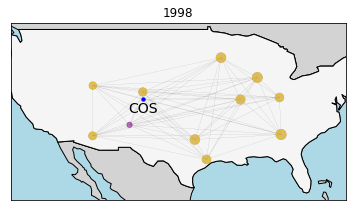
\includegraphics[width=\linewidth]{Exam/Figures/map_COS_98}
        \caption{1998}
    \end{subfigure}
    \hfill
    \begin{subfigure}[t]{0.31\textwidth}
        \centering
        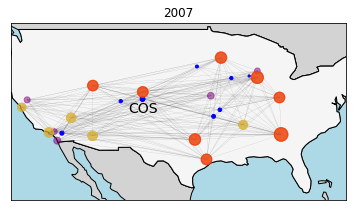
\includegraphics[width=\linewidth]{Exam/Figures/map_COS_07} 
        \caption{2007}
    \end{subfigure}
    \hfill
    \begin{subfigure}[t]{0.31\textwidth}
        \centering
        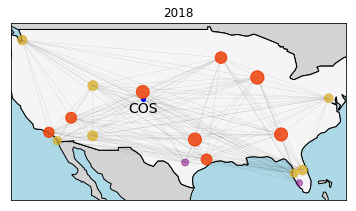
\includegraphics[width=\linewidth]{Exam/Figures/map_COS_18} 
        \caption{2018}
    \end{subfigure}
  \label{fig:map_COS}
\end{figure}
As an alternative measures of centrality in the network, we calculate \textit{betweenness centrality} that measures the degree to which an edge is part of the shortest path between two other edges where path length is defined as the number of traversed links. \\
In the end, we use clustering coefficient, betweenness and degree as features in the prediction model. Note, that these are all node-specific measures, and as such, for each observation, there are two of each corresponding to origin and destination airport. 

% Figur med hhv. degree distribution (til venstre) og betweenness centrality (højre)?
Figure \ref{fig:map_general_18} shows every airport in the network we consider, and the edges that connect them. The network is distributed spatially according to the actual geographical locations of the airports, and overlaid on a map of the continental US. From a visual examination the hub-and-spoke nature of the network is clear. Hubs are somewhat distributed geographically and - at a glance - seem to be placed near population centres. Similar maps of the network in 1998 and 2007 can be found in figures \ref{fig:map_general_98} and \ref{fig:map_general_07} in appendix \ref{app: Network characteristics}. The network seems to have been relatively stable over time; airports that were well connected in 2007 are still well connected in 2018. Table \ref{tab: temporal} shows key characteristics of the network in 1998, 2007 and 2018. The number of airports has risen substantially in the period, as has the number of unique flight routes. The average degree of the network rose from 1998 to 2007, but fell slightly from 2007 to 2018. One should of course keep in mind, that the rise in the number of airports is not necessarily a sign of construction of new airports, but could follow from more carriers, and thereby airports, meeting the inclusion criteria for the dataset.
\begin{table}[H]
\centering 
\caption{Network Characteristics, 1998-2018}
\label{tab: temporal}
\begin{tabular}{|l|l|l|l|}
\hline
\textbf{}                    & \textbf{1998} & \textbf{2007} & \textbf{2018} \\ \hline
Nodes                        & 209           & 310           & 358           \\
Edges                        & 1614          & 2868          & 3220          \\
Average degree               & 15.45         & 18.50         & 18.0          \\
Average shortest path length & -             & 2.31          & 2.38          \\ 
Diameter                     & -             & 5             & 6 
     \\
Clustering Coefficient       & 0.63          & 0.63          & 0.57          \\ \hline
\end{tabular}
\end{table}
Figure \ref{fig:degree_distribution} shows the degree distribution of the network, with a fitted power-law distribution. The hub-and-spoke nature of the network - and the related fact that it is scale-free - is fairly apparent: A large number of nodes have a low degree, while a few nodes have a degree far above the average degree. 
\begin{figure}[H]
  \centering
  \caption{Degree distribution of network, 1998, 2007 and 2018}
    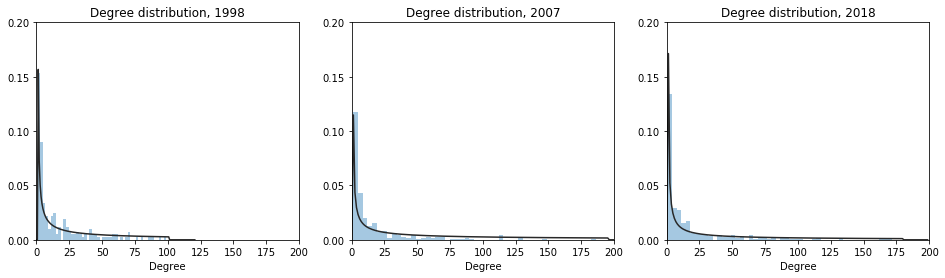
\includegraphics[width=1 \textwidth]{Exam/Figures/degree_distributionv2.png}
  \label{fig:degree_distribution}
\end{figure}
An overview of our three key network characteristics, and how they relate, can be seen in figure \ref{fig:Btwns_CC} in appendix \ref{app: Network characteristics}. Firstly, there is a clear positive relationship between degree and betweenness centrality; airports that are linked to a large number of other airports are also more likely to be part of a shortest path between two airports. This is fairly unsurprising. Secondly, there is no simple relationship between clustering coefficient and either of the other measures. A large number of airports have clustering coefficient equal to 1, implying that all their neighbors are connected to each other. There is also a number of airports with a clustering coefficient of 0, implying that none of their neighbors are connected to each other, or that they only connect to one other airport. 

\subsection{Network vulnerability}
We conduct an analysis of how the network is affected when certain nodes are removed. This analysis is, broadly, in line with the analysis in \cite{chi2004structural}. \\
The figure below shows how key network characteristics (average degree, clustering coefficient and global efficiency) are affected, when nodes are removed. One curve corresponds to removal of the most connected nodes, this is what we refer to as an 'attack' on the network, where the hubs are targeted. \\
Secondly, we consider how the network is affected when we remove the least important nodes first. \\
%Finally, we consider how the network is affected by an event that removes all network in a geographical area (such as might be the case due to natural disaster and extreme weather conditions). We conduct this analysis by choosing a spot in the continental US, calculating the (geographical) distances from each airport to this spot, and then removing all airports within x miles. This final analysis takes advantage of the spatial nature of the network, and provides insight into how geographically determined failures may affect the network. \\
It should be noted, that in this section we analyze the network as it is in our dataset. Obviously, were a number of airports to close for a prolonged period (e.g. due to natural disaster), the agents in the market would make changes to the network to accommodate the new situation. Market forces is likely to have been a determinant in producing the network as is, and exogenous changes to the network would cause changes in behaviour of the agents in the market, that would produce a new network. \\ 

\begin{figure}[H]
  \centering
  \caption{Effect of node removal on average degree (left) and clustering coefficient (right)}
    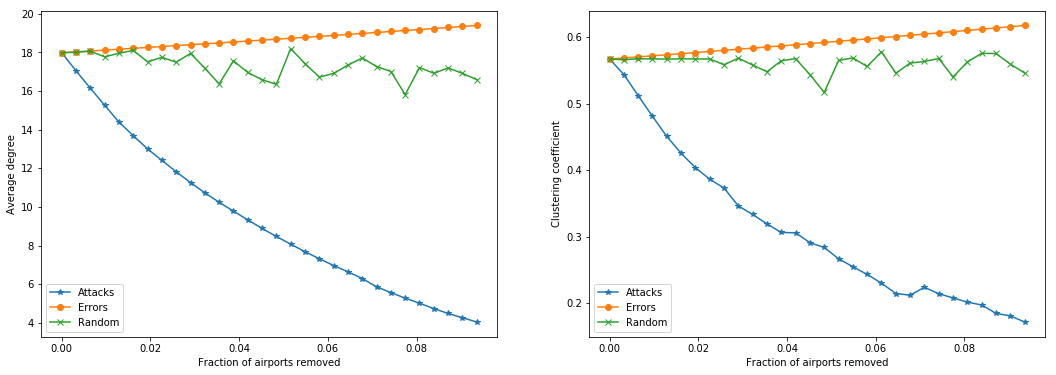
\includegraphics[width=1. \textwidth]{Exam/Figures/attacksanderrors.png}
  \label{fig:attacks_and_errors}
\end{figure}

As the figure shows, the removal of a relatively small number of hubs can dramatically alter network characteristics. Unsurprisingly, removal of the least important nodes increases the measures. The network is thus somewhat vulnerable to 'attacks' on the most connected airports. \\ In the figure, we also show the effect of removing random nodes. Note, that each point represents a "new" network of randomly chosen nodes in the original network. Nodes left out in the first observation may therefore be present in the second observation.  Removal of random nodes has relatively little effect on average degree or the clustering coefficient of the network, again pointing to the fact that the network is vulnerable only to a concerted attack on important hubs. \\ 

\subsection{Predicting Flight Prices - Do Network-related Features add Predictive Power?}
We want to assess whether network characteristics can contribute in predicting flight prices compared to a prediction model using only a set of baseline variables. Our set of baseline variables include: The number of flights on the given route in the year considered, the distance between the two airports, the (average) time in minutes for the flight and the number of carriers who flew the route during the year considered as well as dummies for origin and destination airports. Our set of network-related features includes, for both origin and destination airport: Betweenness centrality, degree and clustering coefficient. \\

In order to get a sense of correlation structure, we show all the continuous variables in the correlation plot in figure \ref{fig:correl}. Unsurprisingly, we see that prices are positively correlated with distance and flight duration and negatively with the number of flights on the route. We see that the rest of the variables, including all our network variables, are only weakly correlated with prices. It is further seen that some of the features exhibit multicollinearity to some degree.

\begin{figure}[H]
  \centering
  \caption{Correlation Plot}
    
\includegraphics[width=0.9 \textwidth]{Exam/Figures/corr_plot.pdf}
  \label{fig:correl}
\end{figure}
In order to predict prices we use a linear prediction model including network characteristics and other things such as distance, flight duration, and airport dummies as predictors. We follow the procedure outline in section \ref{subsec: prediction model}. The procedure is implemented with SKLEARN python module, from which we use \texttt{train\_test\_split}, \texttt{StandardScaler}, \texttt{ElasticNet}, and  \texttt{CVGridSearch}.\footnote{See github for documentation, \url{https://github.com/Morten-Esketveit/TSDS-gruppe-2019/tree/master/Exam}.}


We use a 5-fold cross-validation and for the grid search we allow the L1-ratio to vary between 0.25 and 1, and the alpha parameter to vary between 1 and 20.\footnote{Prior to fitting the model, we scale the features using the StandardScaler in Python. This is done in order to avoid artificially large/small weights which could make convergence difficult when we are using regularization.} 
Figure \ref{fig:validation curve} plots the score, measured in terms of $R^2$ as a function of the regularization parameter $\alpha$ for the three highest L1 ratios. Using grid search the optimal $\alpha$ is approximately 6.2 whereas the optimal L1 ratio is 1. \\ % Læs ovenstående igennem.
\begin{figure}[H]
  \centering
  \caption{Validation Curves}
    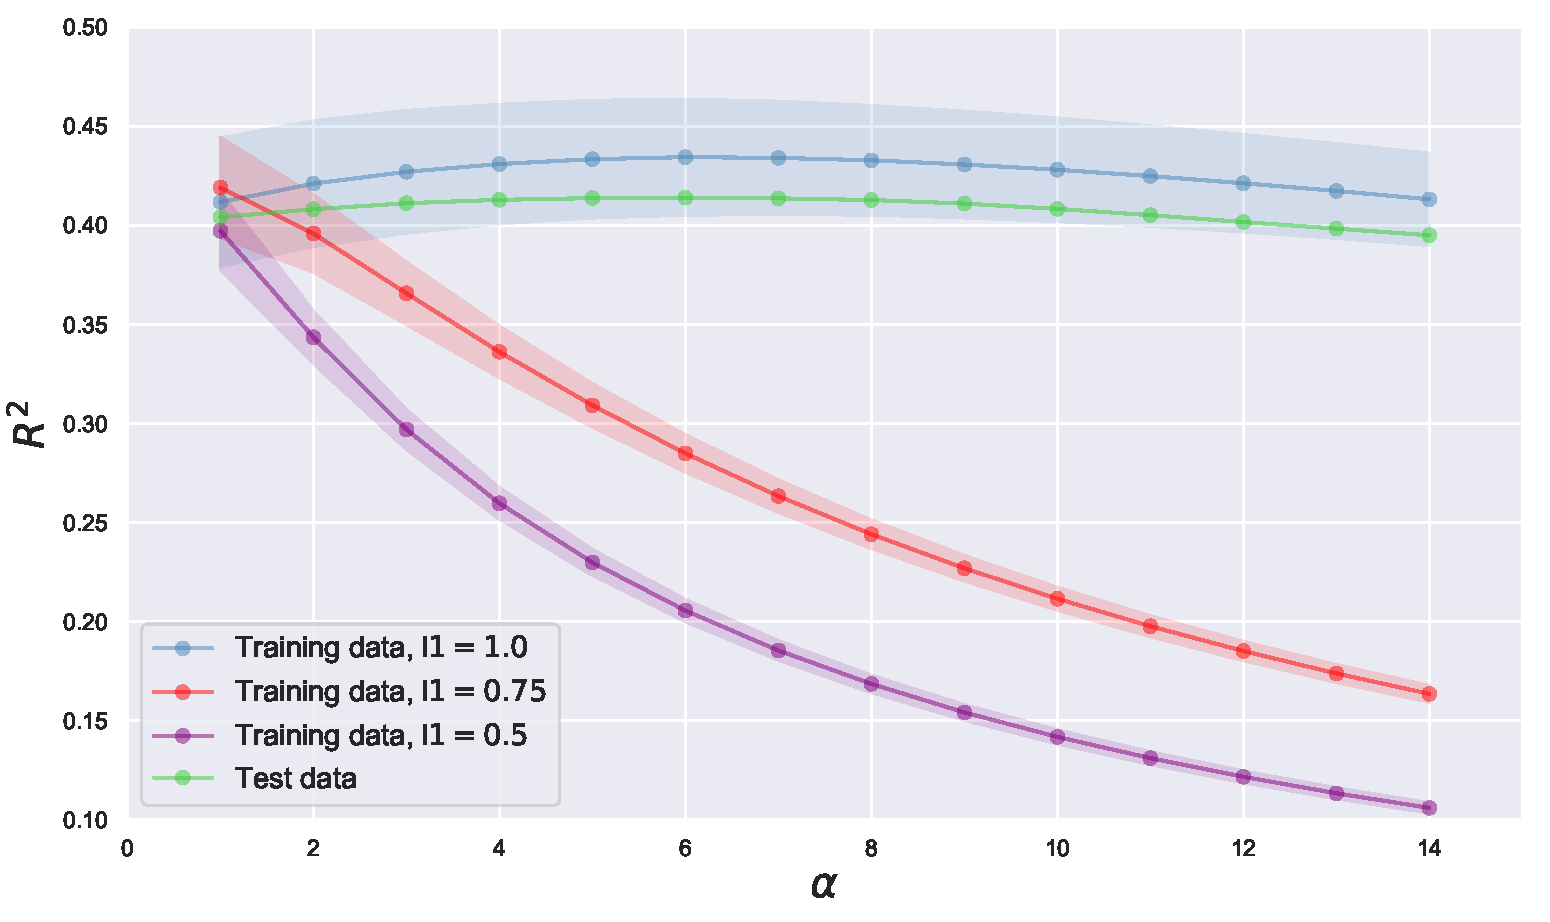
\includegraphics[width=1. \textwidth]{Exam/Figures/validation_curve.pdf}
  \label{fig:validation curve}
\end{figure}
Finally, the best model is tested on our test data and the results are compared to the corresponding model without network features. The results are summarized in table \ref{tab: model1}. Our model is able to explain around 40 pct. of the variation in flight prices. We find, that adding network characteristics only increase the out-of-sample prediction marginally, ie. by 0.5 percentage point. Considering the hyperparametrization both models have a L1 ratio of 1 whereas the $\alpha$ parameter differs slightly. Across the models, the weights of the baseline features are quite similar (see table \ref{tab: coefs} in the appendix) for the number of flights, average time, and the number of flights to and from the destination airport. These are the only continuous baseline features with weights that are different from zero. Among the network  features, origin betweenness and both clustering coefficients enters the model with non-zero weights. Based on the size of the coefficients, the clustering coefficient seems to be the most important, however the regularization tend to bias the coefficients. The way the network features enter the model is a result of the correlation structure showed in figure \ref{fig:correl} and the Lasso regularization. Running the model without airport fixed effects (not shown) increases the importance of network characteristics - the prediction model performs much worse however. In this case, the baseline model is able to explain 15.9 percent of the variation whereas the network model can explain 17.9 percent. 

\FloatBarrier
\begin{table}[htbp]
  \centering
  \caption{Results, Prediction Model}
  \label{tab: model1}
    \begin{tabular}{rlcccc}
    \hline
          &       & \multicolumn{2}{c}{\textbf{Baseline}} & \multicolumn{2}{c}{\textbf{Networks}} \\ 
          &       & \multicolumn{1}{l}{Test data} & \multicolumn{1}{l}{Training data} & \multicolumn{1}{l}{Test data} & \multicolumn{1}{l}{Training data} \\ \hline
    \multicolumn{1}{l}{Model evaluation} & $R^2$  & \multicolumn{1}{c}{0.421} & \multicolumn{1}{c}{0.427} & \multicolumn{1}{c}{0.426} & \multicolumn{1}{c}{0.431} \\
          &       &  &  \multicolumn{1}{c}{(0.026)}     &       & \multicolumn{1}{c}{(0.028)} \\
    \multicolumn{1}{l}{Hyper parameters} & $\alpha$ & \multicolumn{2}{c}{6.359} & \multicolumn{2}{c}{5.872} \\
          & L1 ratio & \multicolumn{2}{c}{1} & \multicolumn{2}{c}{1} \\ \hline
    \end{tabular}%
  \label{tab:addlabel}%
\end{table}%
\FloatBarrier

